%&lualatex
%!TEX TS-program = lualatex
%!TEX encoding = UTF-8 Unicode
% !TeX spellcheck = es-ES
\documentclass[9pt]{beamer}
\setbeamertemplate{section in toc}[sections numbered]
\usepackage{graphicx}
\usepackage[english]{babel}
\usepackage{mathtools}
\usepackage{datetime}
\usepackage{amssymb}
\usepackage[natbib = true, style = alphabetic]{biblatex}
\addbibresource{refs.bib}
\usepackage{physics}
\usepackage{unicode-math}
\usepackage{amsthm}
\setmainfont{CMU Serif}
%--- Cosas de estilo
\usetheme{metropolis}
\metroset{
    sectionpage=progressbar, 
    numbering=fraction, 
    progressbar=foot,
    block=fill
}
\usecolortheme{default}


\setbeamercovered{transparent} %Para que las pausas bajen la opacidad de los elementos en vez de ocultarlos
%--- Para que las demostraciones no ocupen tanto
\setbeamertemplate{proof begin}{
    \vspace{0.5ex}%
    {\usebeamercolor[fg]{block title}\usebeamerfont*{block title}%
    \insertproofname\ }%
}

\setbeamertemplate{proof end}{\par
} %https://tex.stackexchange.com/a/537223/
\addto\captionsspanish{\renewcommand\proofname{Dem.}} %Más corto


%--- Un par de teoremas base



\title{Coisotropic reduction in Multisymplectic Geometry}
\subtitle{Gamma seminar}
\author{Rubén Izquierdo, joint work with Manuel de León.}
\institute{ICMAT}
\date{Wednesday 26 June, 2024}


\theoremstyle{plain} % insert bellow all blocks you want in italic
% to number according to section
\newtheorem{proposition}{Proposition}[section]
\theoremstyle{definition} % insert bellow all blocks you want in normal text
\newtheorem{Def}{Definition}[section] % to number according to section
\newtheorem*{idea}{Proof idea} % no numbered block

%-----------------------------
% Título
%-----------------------------

\begin{document}
\begin{frame}[plain]
    \titlepage
\end{frame}

\begin{frame}{Outline}
    \tableofcontents
\end{frame}



%-----------------------------
% Calculus of Variations
%-----------------------------
%\section{Calculus of Variations}
%\begin{frame}{The variational problem}
Given a fibered manifold $$Y\xrightarrow{\pi} X,$$ we want to find sections $\phi: X \rightarrow Y$ that extremize certain functional (the action) $$S[\phi] := \int_X \mathcal{L}(\phi),$$ where $\mathcal{L}(\phi)$ (the \alert{Lagrangian density}) is an $n$-form on $X$. 

For first order field theories, we can interpret
\begin{align*}
    &\text{Lagrangian dentisy}  \sim \mathcal{L}: J^1 \pi \rightarrow \bigwedge^n X;\\
    &\text{Action} \sim S[\phi] = \int_X \mathcal{L}\circ j^1 \phi.
\end{align*}
\end{frame}

\begin{frame}{Euler-Lagrange equations}
Stationary sections will satisfy $$\dv{t} \bigg |_{t = 0} S[\phi_t] = 0,$$ for every possible variation $\phi_t$, $\phi_0 = \phi.$ The Euler-Lagrange equations for $\phi$ are:
\begin{align*}
    &\alert{\text{Locally}},\,\,\,  \pdv{L}{y^i} = \dv{x^\mu} \left( \pdv{L}{z^i_\mu}\right)\\
    &\alert{\text{Intrinsically}},\,\,\, (j^1\phi)^\ast  \iota_\xi\Omega_{\mathcal{L}} = 0, \forall \xi \in \mathfrak{X}(J^1 Y),
\end{align*}
where $\Omega_{\mathcal{L}}$ is the \alert{multisymplectic form} of the theory, a closed $(n+1)$-form $$\Omega_{\mathcal{L}} = d \left( \pdv{L}{z^i_\mu}\right) dy^i \wedge d^{n-1}x_\mu - \left( \pdv{L}{z^i_\mu}z^i_\mu - L \right) d^n x$$
\end{frame}

\begin{frame}{The importance of multisymplectic geometry}
    \begin{center}
        {\huge Symplectic Geometry $\sim$ Classical Mechanics}\\
        \vspace{1.5cm}
        {\huge Multisymplectic Geometry $\sim$ Classical Field Theory}
    \end{center}
\end{frame}

%-----------------------------
% Bibliography
%-----------------------------
\nocite{deleón2024coisotropic}
\nocite{HamiltonianStructuresIbort}
\nocite{Ibort1999OnTG}
\nocite{deleon2003tulczyjews}
\begin{frame}{References}
    \printbibliography
\end{frame}


%-----------------------------
% Symplectic Geometry
%-----------------------------
\section{Symplectic Geometry}
\begin{frame}{Symplectic manifolds}
   \begin{definition}[Symplectic manifold] A \alert{symplectic manifold} is a pair $(M, \omega)$, where $M$ is a $2n$-dimensional manifold, and $\omega \in \Omega^2(M)$ is a closed, non-degenerate, $2$-form.
   \end{definition}
   \pause
   Thus, for every symplectic manifold we have an isomorphism induced by contraction $$TM \xrightarrow{\flat} T^\ast M; \,\, v \mapsto \iota_v \omega.$$ 
   \pause
   \begin{definition} For a subspace $i: W \hookrightarrow T_x M,$ define the \alert{symplectic orthogonal} as $$W^\perp := \{v \in T_q M, \,\, \omega(v, w) = 0, \forall w \in W \} = \ker i^\ast \circ \flat.$$
   \end{definition}

   $$\alert{\dim W^\perp = 2n - \dim W}$$
\end{frame}

\begin{frame}{Symplectic orthogonal}
\begin{definition} A subspace $W \subseteq T_xM$ (res. submanifold $L$) is called
\begin{itemize}
    \item \alert{isotropic} if $W \subseteq W^\perp$ (res. $T_x L \subseteq (T_x L)^\perp, \forall x \in L$);
    \item \alert{Lagrangian} if $W = W^\perp$ (res. $(T_x L)^\perp = T_x L, \forall x \in L$).
    \item \alert{coisotropic} if $ W^\perp \subseteq W^\perp$ (res. $(T_x L)^\perp \subseteq T_x L, \forall x \in L$).
\end{itemize}
\end{definition}
\pause
A isotropic submanifold is necessarily $n$-dimensional and we have the following characterization:
\begin{proposition} An $n$-dimensional submanifold $i: N \hookrightarrow M$ is Lagrangian if and only if $i^\ast \omega = 0.$
\end{proposition}
\end{frame}

\begin{frame}{Dynamics $=$ Lagrangian submanifolds}
    \begin{definition} Given a function $H \in C^\infty(M)$ define the \alert{Hamiltonian vector field} $X_H \in \mathfrak{X}(M)$ as the unique vector field sastifying $$\iota_{X_H}\omega = dH.$$ A vector field $X \in \mathfrak{X}(M)$ is called \alert{locally Hamiltonian} if $\iota_X \omega$ is closed.
\end{definition}
\pause
With the isomorphism $\flat: TM \rightarrow T^\ast M$ we can define $$\widetilde \omega := \flat ^\ast \omega_M.$$
\begin{theorem} A vector field $X: M \rightarrow TM$ is locally Hamiltonian if and only if it defines a Lagrangian submanifold.
\end{theorem}
\begin{proof} $X(M)$ is Lagrangian if and only if $$0 = X^\ast \widetilde \omega = -d \iota_X \omega.$$
\end{proof}
\end{frame}

\begin{frame}{Coisotropic reduction}
Given a coisotropic submanifold $i:N \hookrightarrow M$, the distribution $$x \mapsto (T_x N)^\perp$$ is regular and involutive. Therefore, it arises from a maximal foliation $\mathcal{F}$.
\pause
\begin{theorem} If $N/\mathcal{F}$ admits a smooth manifold structure such that $\pi: N \rightarrow N/\mathcal{F}$ defines a submersion, then there is an unique symplectic form $\omega_N$ on $N/\mathcal{F}$ such that $$\pi^\ast \omega_N = i^\ast \omega.$$ \alert{Furthermore, if $L$ is a Lagrangian submanifold in $M$, $\pi(L \cap N)$ is a Lagrangian submanifold in $N/\mathcal{F}.$} 
\end{theorem}

Allows for reduction of dynamics!
\end{frame}

\begin{frame}{Coisotropic reduction}
    \begin{proof} We omit the first part. For the projection of Lagrangian submanifolds, let $L$ be a Lagrangian submanifold and denote $L_N := \pi(L \cap N).$\\
    \vspace{0.5cm}

It is
sufficient to see that $\pi(L \cap N)$ is isotropic and that it has maximal dimension in $N / \mathcal{F}$. \pause It is isotropic since $[u] \in
T_q(L _ N)$ implies $\omega_N([u],[v]) = \omega(u,v) = 0$, for every $[v] \in T_q(L _ N)$.\pause  Now, since $\ker d_q\pi =
(T_qN)^{\perp_\omega}$, the kernel-range formula yields \begin{equation}\label{eq1symplectic} \dim L_N = \dim(L \cap N) - \dim (T_q L \cap (T_qN)^{\perp_\omega}). \end{equation} 
Furthermore, \begin{equation}\label{eq2symplectic} \dim(L \cap N) + \dim (T_qL + (T_qN)^{\perp_\omega}) = \dim M,
\end{equation} because $L$ is Lagrangian and $N$ coisotropic. Substituting (\ref{eq2symplectic})in (\ref{eq1symplectic}) we obtain \begin{align} \nonumber
\dim L_N &= \dim M - \dim (T_qL + (T_qN)^{\perp_\omega})- \dim (T_q L \cap (T_qN )^{\perp_\omega}) \\ & \nonumber = \dim M - \dim L - \dim (T_qN)^{\perp_\omega} = \dim M - \dim L -(\dim M - \dim N)\\ &\nonumber = \dim N - \dim L = \dim N - \frac{1}{2} \dim
M, \end{align} which is exactly $\frac{1}{2} \dim N/ \mathcal{F}$, as a direct calculation shows.
    \end{proof}
\end{frame}

\begin{frame}{Poisson bracket and Coisotropic submanifolds}

\begin{definition} For $f, g \in C^\infty(M)$, their \alert{Poisson bracket} is defined as $$\{f,g\} := \omega(X_f, X_g).$$
\end{definition}

We have the following characterization, which is fundamental for the theory of constraints.

\begin{proposition}A submanifold $i: N \rightarrow M$ is coisotropic if and only if, for every pair of functions, $f,g$ constant on $N$, $\{f,g\} = 0$ on $N$.
\end{proposition}
\end{frame}

\begin{frame}{Results to be generalized}
\begin{enumerate}
    \item Endowing $TM$ with the symplectic structure obtained from $\flat: TM \rightarrow T^\ast M$, we can interpret dynamics as Lagrangian submanifolds.
    \pause
    \item Coisotropic submanifolds can be reduced to a symplectic manifold.
    \pause
    \item Lagrangian submanifolds project onto Lagrangian submanifolds under this reduction
    \pause
    \item Coisotropic submanifolds can be characterized by the Poisson bracket.
\end{enumerate}    
\end{frame}

%-----------------------------
% Multisymplectic Manifolds
%-----------------------------
\section{Multisymplectic Manifolds}
\begin{frame}{Multisymplectic Manifolds}
    \begin{definition} A \alert{multisymplectic manifold} of order $k$ is a pair $(M, \omega)$, where $M$ is a smooth manifold, and $\omega$ is a closed $(k+1)-$form.
    \end{definition}
    \alert{No non-degeneracy required.\\
    }
    \pause
    Now we have a collection of maps $$\bigvee_ q M \xrightarrow{\flat_q} \bigwedge^{k+1-q} M; \,\, U \mapsto \iota_U \omega$$ which endow $\bigvee_q M$ with a multisymplectic structure $$\widetilde \Omega^q_M := \flat_q^\ast  \Omega^{k+1-q}_M,$$ where $\Omega^{k+1-q}_M$ is the canonical multisymplectic structure on $\bigwedge^{k+1-q} M$.
\end{frame}

\begin{frame}{Multisymplectic manifolds}
    \begin{definition} For $W \subseteq T_x M,$ and $1 \leq j \leq k$ define the \alert{multisymplectic orthogonal} as $$W^{\perp, j}:= \{v \in T_x M: \,\, \iota_{v \wedge w_1 \wedge \cdots w_j} \omega = 0, \,\, \forall w_1, \dots, w_j \in W\}.$$
    \end{definition}
    \pause
    
    \begin{Def} We will say that a subspace $W \subseteq T_x M$ is 
    \begin{itemize}
    \item \alert{j-isotropic}, if $$W  \subseteq W^{\perp, j};$$
        \item \alert{$j$-coisotropic}, if $$W^{\perp,j} \subseteq W + \ker \flat_1;$$
        \item \alert{$j$-Lagrangian}, if $$W^{\perp, j} = W + \ker \flat_1.$$
    \end{itemize}
    \end{Def}
     These definitions extend in the natural way to submanifolds.
\end{frame}
\begin{frame}{Form bundle}
    Fix a manifold $L$ and define $$M := \bigwedge^k L.$$ If we define the \alert{tautological $k$-form} $$\Theta_L |_{\alpha} (v_1, \dots, v_k) = \alpha(\pi_\ast v_1, \dots, \pi_\ast v_k),$$ then $$\Omega_L := d \Theta_L$$ defines a canonical non-degenerate multisymplectic structure on $\bigwedge^k L.$ \pause  In canonical coordinates $(x,p_{i_1, \dots, i_k})$ representing the form $$\alpha = p_{i_1, \dots, i_k} \wedge dx^{i_1} \wedge \cdots \wedge d x^{i_k},$$ \pause the canonical multisymplectic form reads $$\Omega_L = dp_{i_1, \dots, i_k} \wedge dx^{i_1} \wedge \cdots \wedge d x^{i_k}.$$
\end{frame}

\begin{frame}{An useful lemma}
\begin{lemma} Let $(V, \omega)$ be a $k$-multisymplectic manifold and $U, W$ be $k$-isotropic and $1$-isotropic subspaces respectivley such that $$V = U \oplus W.$$ Then, $U$ is $k$-Lagrangian.
\end{lemma}
\begin{proof} Let $u + w \in U^{\perp, k},$ for $u \in U$, $w \in W$. Then, for all $u_1, \dots, u_k \in U$ we have $$\omega(u + w, u_1, \dots, u_k) = \omega(w, u_1, \dots, u_k) = 0.$$ We claim that $w \in \ker \flat_1.$ \pause Indeed, given $u_i + w_i \in V$, $$\omega(w, v_1, \dots, v_k) = \omega(w, u_1 + w_1, \dots, u_k +w_k) = \omega(w, u_1, \dots, u_k) = 0,$$ where in the last equality we used that $W$ is $1$-isotropic. Therefore, if $u + w \in U^{\perp, k},$ we have $$u + w \in U +\ker \flat_1,$$ that is $$U^{\perp, k} \subseteq U + \ker \flat_1,$$ proving that $U$ is $k$-coisotropic and, therefore, $k$-Lagrangian
\end{proof}
\end{frame}

\begin{frame}
\begin{proposition}
        A differential $k$-form $$\alpha: L \rightarrow \bigwedge^k L$$ defines a $k$-Lagrangian submanifold if and only if it is closed.
\end{proposition}
\begin{proof} Since the vertical distribution of $L \rightarrow \bigwedge^k L$, $W$, defines a $1$-Lagrangian distribution, and $\alpha(L)$ is always complementary to $W$, it is enough to show that $\alpha$ is $k$-isotropic. We have $$\alpha^\ast \Omega_L = d \alpha,$$ which ends the proof.
\end{proof}
\end{frame}


%-----------------------------
% Interpretation of Hamiltonian multivectorfields
%-----------------------------
\section{Hamiltonian multivector fields and forms}
\begin{frame}{Hamiltonian multivector fields and forms}
\begin{definition} Let $(M, \omega)$ be a multisymplectic manifold of order $k.$ A multivector field $$U: M \rightarrow \bigvee_q M$$ is called \alert{Hamiltonian} if there exists a $(k-q)$-form $$\alpha: M \rightarrow \bigwedge^{k-q} M$$ such that $$\iota_U \omega = d \alpha.$$ We refer to $\alpha$ as the \alert{Hamiltonian form.} When $\iota_U \omega$ is closed, we call $U$ \alert{locally Hamiltonian}.
\end{definition}
\end{frame}

\begin{frame}{Bracket of Hamiltonian forms}
We will denote by the quotient of all Hamiltonian forms $(\Omega_H(M))$ by the space of all closed forms ($Z(M)$) $$\widehat{\Omega}_H(M) := \Omega_H(M)/Z(M).$$
\pause
Defining $$\deg [\alpha] := k - 1 - (\text{order of }\alpha),$$ and $$\{[\alpha], [\beta]\}^\bullet = -(1)^{\deg \alpha +1 }[\iota_{U \wedge V} \omega],$$ where $$\iota_ U \omega = d \alpha, \iota_V \omega = d \beta,$$
we have 
\pause
\begin{theorem}
     For every multisymplectic manifold, $(\widehat{\Omega}_H(M), \{\cdot, \cdot\}^\bullet)$ is a graded Lie algebra. 
\end{theorem}
In particular,
\begin{proposition} $(\widehat{\Omega}^{k-1}_H(M), \{\cdot, \cdot\}^\bullet)$ is a Lie algebra.
\end{proposition}
\end{frame}

\begin{frame}{Bracket of Hamiltonian forms}
    Let us restrict our attention to \alert{currents} ($(k-1)$-forms). Defining (without quatienting) $$\{\alpha, \beta\} = \iota_{U \wedge V}\omega,$$ $\{ \cdot , \cdot \}$ does not satisfy the Jacobi identity. \pause 
   Nevertheless, $$\{\alpha, \{\beta, \gamma\}\} + \text{cycl.} = d \iota_{U \wedge V \wedge W} \omega.$$
 This gives an $L_\infty-$algebra structure on $$\Omega^0(M) \xrightarrow{d} \cdots \xrightarrow{d} \Omega^{k-2}(M) \xrightarrow{d} \Omega^{k-1}_H(M).$$
\end{frame}


\begin{frame}{Dynamics = Lagrangian submanifolds}
\begin{theorem}[\cite{deleón2024coisotropic}] A mutivector field $U: M \rightarrow \bigvee_q M$ is locally Hamiltonian if and only if it defines a $(k+1-q)-$Lagrangian submanifold.
\end{theorem}
\pause
\begin{proof}
Since $U(M)$ defines a $(k+1-q)-$isotropic submanifold, it follows from the decomposition $$T \bigvee_q M \bigg |_{U(M)} = T U(M)  \oplus \widetilde W^{k+1-q},$$ where $\widetilde{W}^{k+1-q}$ is $1$-isotropic.
\end{proof}
\end{frame}


%-----------------------------
% Coisotropic submanifoldS
%-----------------------------
\section{Coisotropic submanifolds}
\begin{frame}{Coisotropic submanifolds and brackets}
\begin{proposition} If $i: N \hookrightarrow M$ is a $k$-coisotropic submanifold, the subspace of $(k-1)$-forms wich are closed on $N$, $$I_N = \{ [\alpha] \in \Omega^{k-1}_H(M): \,\, d \alpha = 0\, \text{ on } N\}$$ defines a subalgebra of the Lie algebra $\widehat \Omega_H^{k-1}(M).$
\end{proposition}
\pause
\begin{proof}
Let $\widehat{\alpha}, \widehat{\beta} \in \widehat{I}_N.$ Then, there are vector fields $X_\alpha, X_\beta$ satisfying $$\iota_{X_\alpha} \omega = d \alpha, \,\, \iota_{X_\beta} \omega = d \beta.$$ Since $i^\ast d\alpha, i^\ast d\beta = 0,$ we conclude that $X_\alpha, X_\beta$ take values in $(TN)^{\perp, k} \subseteq TN + \ker \flat_1.$ Without loss of generality, we can assume that $X_\alpha$, $X_\beta$ take values in $TN$. Now, since $$\{\widehat{\alpha}, \widehat{\beta}\}^\bullet =  (-1)^{(k-1)} \widehat{ \iota_{X_\alpha \wedge X_\beta} \omega},  i^\ast \left(\iota_{X_\alpha \wedge X_\beta} \omega\right) = 0,$$ concluding that $$\{\widehat{\alpha}, \widehat{\beta}\}^\bullet \in \widehat{I}_N.$$
\end{proof}
\end{frame}

\begin{frame}{Coisotropic reduction}
    Given a $k$-coisotropic submanifold $i: N \hookrightarrow M,$ we have
\begin{proposition} The distribution $x \mapsto (T_x N)^{\perp, k} \cap T_xN \subseteq T_xN$ is involutive.
\end{proposition}
Thus, when it is regular, there exists a foliation consisting of maximal leaves of the distribution, $\mathcal{F}.$ \pause Then,
\begin{theorem} When $N/\mathcal{F}$ admits a smooth manifold structure such that the projection $\pi: N \rightarrow N/\mathcal{F}$ defines a submersion, there exists an unique multisymplectic form $\omega_N$ on $N/\mathcal{F}$ such that $$\pi^\ast \omega_N = i^\ast\omega.$$
\end{theorem}
\alert{What about projection of Lagrangian submanifolds?}
\end{frame}


\begin{frame}{Multisymplectic manifolds of type $(k,r)$} 
\begin{definition}
    Let $L$ be a manifold and $\mathcal{E}$ be a regular distribution on $L$. Define:
$$\bigwedge^k_r L = \{ \alpha \in \bigwedge^k L: \,\, \iota_{e_1 \wedge \cdots \wedge e_r} \alpha = 0, \forall e_1, \dots, e_r \in \mathcal{E}\}.$$
\end{definition}
\pause
\begin{proposition} $(\bigwedge^k_r L, \Omega_L)$ is a non-degenerate multisymplectic manifold, where $\Omega_L$ is (the restriction of the) canononical multisymplectic form.
\end{proposition}
These are the type of multisymplectic manifolds that appear in the study of Classical Field Theories, with $r= 2.$
\end{frame}

\begin{frame}{Multisymplectic manifolds of type $(k,r)$}
\begin{definition} A \alert{multisymplectic manifold} of type $(k,r)$ is a tuple $(M, \omega, W, \mathcal{E}),$ where $(M,\omega)$ is a non-degenerate multisymplectic manifold, $W$ is a regular, integrable, $1$-Lagrangian distribution, and $\mathcal{E}$ is a subbundle of $TM/W$ satisfying
\begin{itemize}
    \item[a)]$\iota_{e_1 \wedge \cdots \wedge e_r} \omega = 0,$ for all $e_i \in TM$ such that $e_i + W \in \mathcal{E};$
    \item[b)] $$\dim \bigwedge^k_r T_qM/ W_q = \dim M.$$
\end{itemize}
\end{definition}
\pause
\begin{theorem} A multisymplectic manifold of type $(k,r)$ $(M, \omega, W, \mathcal{E})$ is locally multisymplectomorphic to $\bigwedge^k_r L$.
\end{theorem}
\end{frame}
\begin{frame}{An example of coisotropic reduction}
    Let $L$ be a smooth manifold, $i: Q \subseteq L$ be a submanifold, and $\mathcal{E}$ be a regular distribution. \pause Then,

    \begin{proposition} $N := \bigwedge^ k_r L \big |_Q$ defines a $k$-coisotropic submanifold, and for $\alpha \in N$, $$\left( T_{\alpha}N\right)^{\perp, k} \cong 0 \oplus \ker i^\ast,$$ where $$i^\ast: \bigwedge^k_r L \rightarrow \bigwedge^k_r Q$$ is the restriction. Here, the vertical forms are taken with respect to $\widetilde{\mathcal{E}} = \mathcal{E} \cap TQ$ (not necessarily of constant rank).
    \end{proposition}
\end{frame}
\begin{frame}{An example of coisotropic reduction}
    \begin{proof} ($r = 0$ for symplicity) To prove the previous equality, we just need to prove it in the linear case $$U \oplus \bigwedge^k L^\ast \subseteq L \oplus \bigwedge^k L^\ast.$$ Let $(v, \alpha) \in (U \oplus \bigwedge^k L^\ast) ^{\perp, k}.$ Then,
    \begin{enumerate}
        \item  $0 = \Omega_L((v, \alpha), (0, \beta), (u_2, 0), \dots, (u_k, 0)) = \beta(v, u_2, \dots, u_k),$ which implies $v = 0$.\pause
        \item $0 = \Omega_L((v, \alpha), (u_1,0), \dots, (u_k, 0)) = \alpha(u_1, \dots, u_k),$ which implies $$\alpha \in \ker i^\ast.$$
    \end{enumerate}
    \end{proof}
\end{frame}

\begin{frame}{An example of coisotropic reduction}
When $\widetilde{\mathcal{E}} = \mathcal{E} \cap Q$ has constant rank, $(TN)^{\perp, k}$ has constant rank and thus, is an involutive distribution. For $x \in Q$, the leaf through $(x, 0) \in N$ is $$\ker \left(i^\ast:\bigwedge^k_r T_x^\ast L \rightarrow \bigwedge^k_r T^\ast_x Q\right).$$ Therefore,
\pause
\begin{theorem} For $N = \bigwedge^k_r L \big |_Q$, where $TQ \cap \mathcal{E}$ has constant rank, $$N/\mathcal{F} \cong \bigwedge^k_r Q.$$ Furthermore, the multisymplectic structure induced on the quotient is the natural multisymplectic structure.
\end{theorem}
\end{frame}

\begin{frame}{Projection of Lagrangian submanifolds (example)}
Define a Lagrangian submanifold through a closed form $$\alpha: L \rightarrow \bigwedge^k_r L.$$ Then, the projection to the quotient $$\pi(\alpha(L) \cap N); \,\, \pi: N \rightarrow N/\mathcal{F}$$ is the image of $$i^\ast\alpha:  Q \rightarrow \bigwedge^k_r Q,$$ which is Lagrangian, because $i^\ast \alpha$ is closed as well.
\pause
\begin{theorem} In our example, Lagrangian submanifold transversal to the vertical distribution reduce to Lagrangian submanifolds.
\end{theorem}
\end{frame}

\begin{frame}{Local characterization of vertical coisotropic submanifolds}
    \begin{definition} Let $(M, \omega, W, \mathcal{E})$ be a multisymplectic manifold of type $(k,r).$ A submanifold $i:N \hookrightarrow M$ is called \alert{vertical} if $W|_N \subseteq TN.$
    \end{definition}
    \pause
    \begin{theorem}[\cite{deleón2024coisotropic}] Let $(M, \omega, W, \mathcal{E})$ be a multisymplectic manifold of type $(k,r)$, $i: N \hookrightarrow M$ be a vertical $k$-coisotropic submanifold, and $j:L \hookrightarrow M$ be a $k$-Lagrangian submanifold complementary to $W$. Then there is a neighborhood $U$ of $L$ in $M$, a submanifold $Q \hookrightarrow L,$ a neighborhood $V$ of $L$ in $\bigwedge^k_r L,$ and a multisymplectomorphism $$\phi: U \rightarrow V$$ satisfying
    \begin{itemize}
        \item[a)] $\phi$ is the identity on $L;$
        \item[b)] $\phi(N \cap U) = \bigwedge^k_r L \big |_Q \cap V.$
    \end{itemize}
    \end{theorem}
\end{frame}
\begin{frame}{Local characterization of Lagrangian submanifolds}
    \begin{theorem}[Normal form of Lagrangian submanifolds \cite{deleon2003tulczyjews}] Let $(M, \omega, W, \mathcal{E})$ be a multisymplectic manifold of type $(k,r)$, $j:L \hookrightarrow M$ be a $k$-Lagrangian submanifold complementary to $W$. Then there is a neighborhood $U$ of $L$ in $M$, a neighborhood $V$ of $L$ in $\bigwedge^k_r L,$ and a multisymplectomorphism $$\phi: U \rightarrow V$$ satisfying
        \begin{itemize}
            \item[a)] $\phi$ is the identity on $L;$
            \item[b)] $\phi( U) =  V.$
        \end{itemize}
        \end{theorem} 
\end{frame}
\begin{frame}{Idea of the proof of local form of coisotropic submanifolds}
    \begin{enumerate}
        \item Take $$\phi: U \rightarrow V$$ the multisymplectomorphism of the previous local form, where $$L \subseteq U \subseteq M; \,\, L \subseteq V \subseteq \bigwedge^k_r L.$$

        \item Define $Q:= \phi(L \cap N).$

        \item Since $\phi$ preserves the vertical distributions, it also preserves their leaves and then, $$\phi(U \cap N) = \bigwedge ^k_r L \big |_ Q \cap V.$$
        \begin{figure}
            \centering
            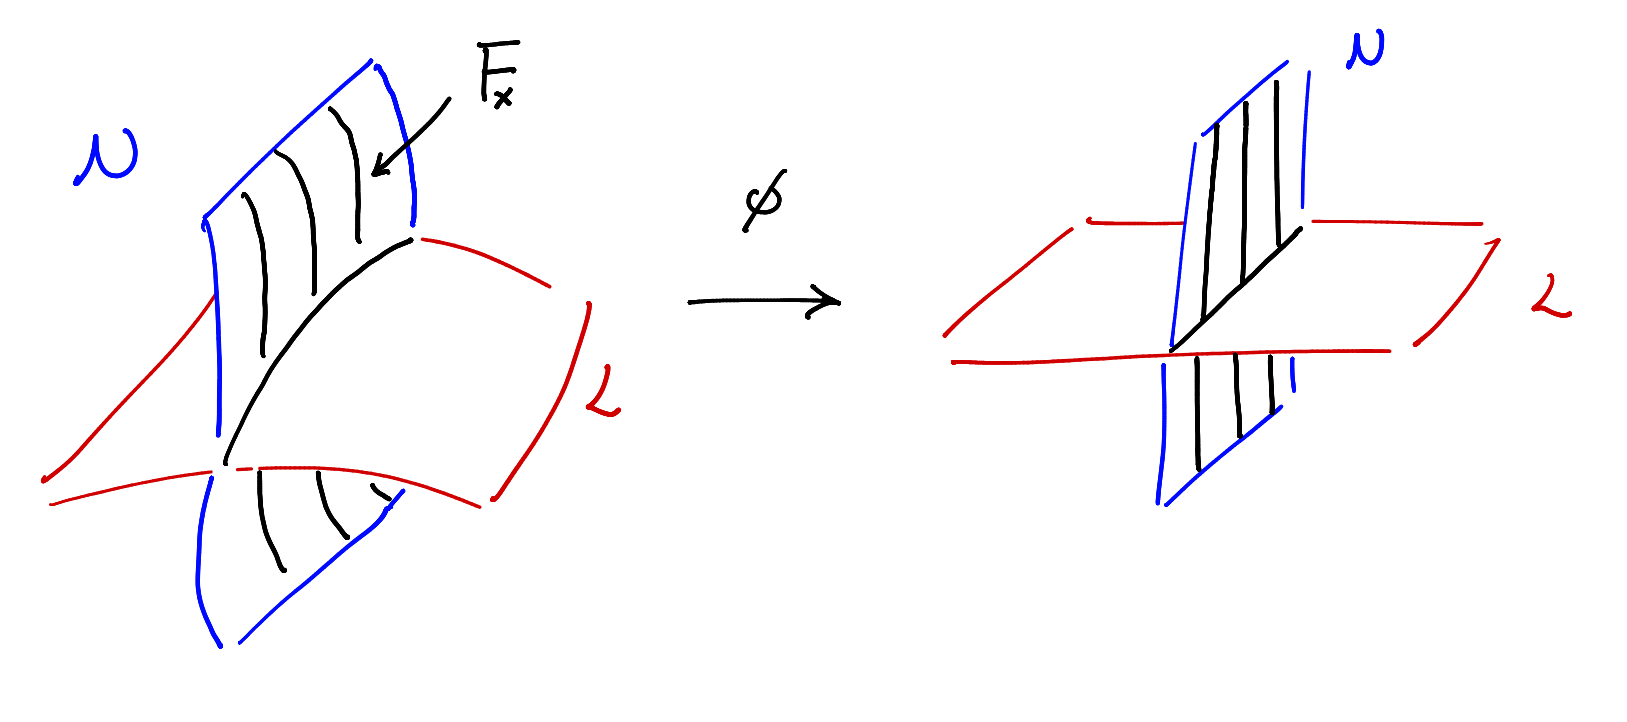
\includegraphics[scale = 0.2]{theorem.PNG}
        \end{figure}
    \end{enumerate}
\end{frame}

\begin{frame}{Lagrangian submanifold projection}
This local characterization allows us to prove:
\begin{theorem}[\cite{deleón2024coisotropic}] Let $(M, \omega, W, \mathcal{E})$ be a multisymplectic manifold of type $(k,r),$ $i: N \hookrightarrow M$ be a vertical $k$-coisotropic submanifold, and $j: L \hookrightarrow M$ be $k$-Lagrangian submanifold complementary to $W$. If $TN / W \cap \mathcal{E}$ has constant rank, so does $(TN)^{\perp, k}$ and we have that, denoting by $\pi: N \rightarrow N/\mathcal{F}$ the canonical projection, \alert{$\pi(L \cap N)$ is Lagrangian in $(N, \omega_N)$}.
\end{theorem}

A general result is not possible, since we can easily find counterexamples.
\end{frame}

\begin{frame}{A counterexample}
Let $L = \langle l_1, l_2, l_3\rangle$ be a $3$-dimensional vector space and define $$V:= L \oplus \bigwedge^2 L^\ast.$$ Let $l^1, l^2, l^3$ be the dual basis induced on $L^\ast$ and denote $$\alpha^{ij} := l^i \wedge l^j.$$ Then $$V = \langle l_1, l_2, l_3, \alpha^{12}, \alpha^{13}, \alpha^{23}\rangle.$$ Let $l^1, l^2, l^3, \alpha_{12}, \alpha_{13}, \alpha_{23}$ be the dual basis. We have $$\Omega_L = \alpha_{12} \wedge l^1 \wedge l^2 + \alpha_{13} \wedge l^1 \wedge l^3 + \alpha_{23}\wedge l^2 \wedge l^3.$$ Define $$N := \langle l_1 + l_2, l_1 + \alpha^{23}, l_2 + \alpha^{13}, l_3, \alpha^{12}\rangle.$$ 

\end{frame}
\begin{frame}{A counterexample}
Then $N$ is a $2$-coisotropic subspace. Indeed, a quick calcultion shows $N^{\perp, 2} = 0$. This implies that the quotient space $N/N^{\perp, 2}$ is (isomorphic to) $N.$ Now, taking as the $2$-Lagrangian subspace $L = \langle l_1, l_2,l_3\rangle$, we have $$L \cap N = \langle l_1 + l_2 , l_3 \rangle.$$ However, this does not define a $2$-Lagrangian subspace of $(N, \Omega_L |_N)$, since $\alpha^{12} \in (N \cap L)^{\perp, 2}$, but $ \alpha^{12} \not \in(L \cap W).$
    
\end{frame}



%-----------------------------
% Final remarks
%-----------------------------
\section{Final remarks and future research}
\begin{frame}{Final remarks and future research}
\begin{itemize}
    \item We gave an interpretation of dynamics as Lagrangian submanifolds.
    \item We proved a coisotropic reduction theorem in a particular class of multisymplectic manifolds.
    \item For future research we have proposed the following: 
    \begin{itemize}
        \item Apply the results obtained to Field Theories (regularization, constraint analysis, etc)
        \item Extend these results to multicontact geometry for the study of dissipative fields.
    \end{itemize}
\end{itemize}
\end{frame}



\begin{frame}
\begin{center}
    {\Huge Thank you for your attention!}\\
    \vspace{1 cm}
    {\Huge Questions?}
\end{center}
\end{frame}

\end{document}